\chapter{Introduction} \label{chap:introduction}

	Over the years, nuclear science and technology has made many positive contributions towards improving the quality-of-life of millions of people. Nuclear provides the world's second-largest source of low-carbon energy but it also helps control the spread of diseases, assists in diagnosis and treatment of cancer, powers space exploration missions, and drives the advancement of industry, agriculture and technology. Nuclear energy is not only at the core of world's sustainable development efforts but is also poised to take on an even bigger role as the world collectively moves to decarbonise many hard-to-abate sectors of the economy. 

	As of 2022, around 440 nuclear plants around the world supplied \SI{2653}{\tera\watt\hour} of electricity, around 10\% of the world's total electricity \cite{WNA:2019aa}. Despite the strong support for, and growth in, intermittent renewable electricity sources in recent years, the fossil fuel contribution to power generation has remained virtually unchanged over the last decade and a half \cite{WNA:2019aa}. In its World Energy Outlook 2021, the Organisation for Economic Co-operation and Development (OECD) International Energy Agency (IEA)  has proposed an ambitious \emph{Sustainable Development Scenario} consistent with the goals clean and reliable energy and a reduction of air pollution, among other aims. In the scenario, by year 2050, nuclear based electricity generation should increase by 75\% to \SI{4714}{\tera\watt\hour}, a  capacity growth to \SI{669}{\giga\watt\electric} \cite{IEA:2018aa}. Key to a sustained growth of nuclear power is demonstrating their safety, reliability and economy.
	
	Though many nations across the globe, both industrialised and developing, are confident of the potential of nuclear energy, several challenges related to sustainability, reliability, economic competitiveness, safety, risk of proliferation, anticipated future needs beyonds electricity, and need for government support  remain \cite{GIF:2009aa}. To meet these challenges and develop future nuclear energy systems, the Generation {IV} International Forum (GIF) is undertaking necessary research and development to develop the next generation of innovative nuclear energy systems that can supplement today's nuclear plants and transition nuclear energy into the long term \cite{GIF:2019aa}. While promising in terms of sustainability, economics, safety and reliability, and proliferation resistance and physical protection, the Generation {IV} nuclear reactors pose unique challenges in terms of engineering design, modelling and construction of these reactors. The design issues are themselves quite complicated and span a wide array of knowledge domains such reactor physics, chemistry, materials science, fluid flow and heat transfer, etc. Safe and economical operation of any nuclear system relies heavily on the success of nuclear fuels and structural materials which must operate under extreme environments. Compared to current generation of reactors, advanced reactors will operate at higher temperatures, under higher irradiation, at higher pressures, and in some cases, like Molten Salt Reactors (MSRs), with fluids that present more challenging corrosion problems \cite{Allen:2010aa}.

%==============================================================================================================================
%												Challenges in Nuclear Material Design
%==============================================================================================================================	
\section{Material Challenges in Nuclear Systems}
	Design and discovery of materials most suited for a specific application is an intrinsic part of development of new technology as many engineering designs can only be as good as the materials available during design and innovation. In conventional materials, the mechanical, thermophysical and chemical properties are often of main interest but nuclear materials must overcome significant challenges to provide the desired levels of reliability and safety commensurate to strict quality assurance requirements. Nuclear reactors present extreme environments for components irrespective of the reactor technology and not only do materials need to meet the physical and chemical performance requirements, but must also demonstrate desirable nuclear physics characteristics. The core in particular presents an exceptionally harsh environment of high temperature, high pressure, high stresses, intense radiation and a chemically aggressive environment and the properties desirable from a nuclear perspective, such as high power density, exert high operational burdens on fuels and structural materials \cite{Zinkle:2013aa}.  As advanced reactor designs gain increasing traction, the material-challenges are only going to get worse. Advanced reactors, such as Molten Salt Reactors, operate not only at higher temperature, pressure and irradiation flux but also with coolants that present more challenging corrosion problems than the current lot of Light Water Reactors (LWRs) and Heavy Water Reactors \cite{Allen:2010aa}. Moreover, Generation {IV}  reactors are expected to have a longer operating time of at least sixty years. Some of the materials challenges are as follows:
	\begin{itemize}
		\item Nuclear materials must satisfy the standard design requirements like tensile properties, thermal creep, cyclic fatigue and creep fatigue but such properties are significantly affected by degradation mechanisms resulting from radiation damage. Bulk radiation leads to  low temperature radiation hardening and embrittlement, solute segregation and phase stability, irradiation creep, void swelling and high temperature helium embrittlement \cite{Olander:76,Was:2017aa}.
		\item The LWR cores must behave well under mechanical stress, irradiation and corrosion due to hot water and steam. pH control and scavenging of radiolysis products has significant impact on corrosion, stress-corrosion cracking and CRUD formation.
		\item Extended operation and new operating regimes pose a new challenge as new degradation mechanisms due to corrosion or ageing may be revealed. This adds an extra layer of uncertainty to the material design and discovery process.
		\item Behaviour of oxide fuels interacting with \ce{Zr} alloys under irradiation conditions is still an area of open research. Hydrogen/deuterium uptake and radiation induced hardening can compromise the cladding's resistance to pellet-cladding interaction under reaction-induced accident scenarios. In loss of coolant accident type scenarios, \ce{Zr} oxidation can rapidly degrade cladding material properties.
		\item In advanced LWRs such as small modular reactors (SMRs), advanced manufacturing techniques, such as additive manufacturing, may be deployed but it would be important to compare the impact of microstructural difference on bulk material properties.
		\item In advanced reactors such as MSR, sodium-cooled fast reactor (SFR), and lead-cooled fast reactor (LFR), there will be an increased emphasis on strength, creep and creep-fatigue behaviour due to very high radiation damage driven by void swelling and phase stability.
		\item In high-temperature, high-dose advanced reactors, chemical interaction between coolant and structural materials will result in additional degradation mechanisms. In particular, corrosion of molten salt-facing structural materials in MSRs is expected to cause significant leaching and deposition.
	\end{itemize}
	
%==============================================================================================================================
%														Thermochemistry
%==============================================================================================================================	
\section{Thermochemistry in Nuclear Systems}
	Thermochemistry and principles of computational thermodynamics play a key role in nuclear material modelling. Since nuclear materials are continuously evolving due to transmutations and fission product generation, so do their material properties. The laws of thermodynamics govern many phenomena in nuclear materials and are important for applications such as understanding phase equilibria, which affects nucleation and dissolution of phases, oxidation potential of cladding, thermochemical properties of fuels and many others. As such, thermodynamic principles are sufficient for predicting many phenomena and are, at a minimum, imperative to understanding more complex and dynamic physics. Some of the key applications of thermodynamics that make it an indispensable part of material design and discovery process include but are not limited to:
	\begin{enumerate}
		\item Understanding the fuel and cladding composition and microstructure, manufacturing and design of fuel and cladding materials, and prediction of thermal stability of fuel and cladding materials.
		\item Understanding fission product chemistry and their effect on material properties.
		\item Predicting chemical interactions between fuel and cladding materials and coolant.
		\item Source term analyses and predicting phases that form between reactor materials under severe accident scenarios.
		\item Optimising fuel salt composition and predicting impact of impurities on molten salt corrosion in MSRs.
	\end{enumerate}
	
	While the concepts of thermodynamics can be embodied in both non-equilibrium and equilibrium descriptions, it is often thermodynamic equilibrium that is leveraged in applications. Even when the materials are, in many cases, in non-equilibrium conditions, an understanding of the phases that shall form under equilibrium conditions provides valuable knowledge as it gives the direction of evolution of the system.  In fact, in nuclear materials, the high temperature conditions lead to a rapid approach to equilibrium and under suitable conditions, make equilibrium thermodynamics a suitable approximation.
	
%==============================================================================================================================
%													Modelling and Simulation
%==============================================================================================================================	
\section{Modelling and Simulation}
	Modern materials, including nuclear materials are developed using a combination of discovery, which involves evaluating existing materials to identify candidates with desirable properties, and design, which aims at  creating new materials with predefined qualities \cite{STAN200920}. While the traditional approach to discovery and design of materials was almost entirely experimental, recent developments in modelling and high performance computing have resulted in a much stronger collaboration and integration among theory, experiments and computational science. Multiscale, multiphysics models and simulations enable investigations over  a wide range of length and time scales which would otherwise be unfeasible using only experiments. Thus, computational models help augment and guide experimental campaigns and support economical discovery and design of materials within reasonable lead times.

	 Nuclear materials are subjected to extreme radiation environments that continuously complicate the physics and chemistry, and alter the thermo-mechanical properties of the material \cite{STAN200920}. Complex interactions between the different physical phenomena occurring in the materials are often very tightly coupled and many important aspects are inherently multidimensional  as well \cite{WILLIAMSON2012149}. As an example, one can consider MSRs where, as shown in figure~\ref{fig:msr_mf}, multiple physics  are required for understanding the behaviour and for predicting phenomena such as mass accountancy. Another aspect to consider is that of the different time and length-scales involved with length-scales ranging from inter-atomic spacing to meters, and time-scales ranging from microseconds to years. For example, radiation defects start within picoseconds at the atomistic scales and propagate to larger length-scales over time-scales which are several magnitudes longer.
	\begin{figure}[htb]
		\centering
		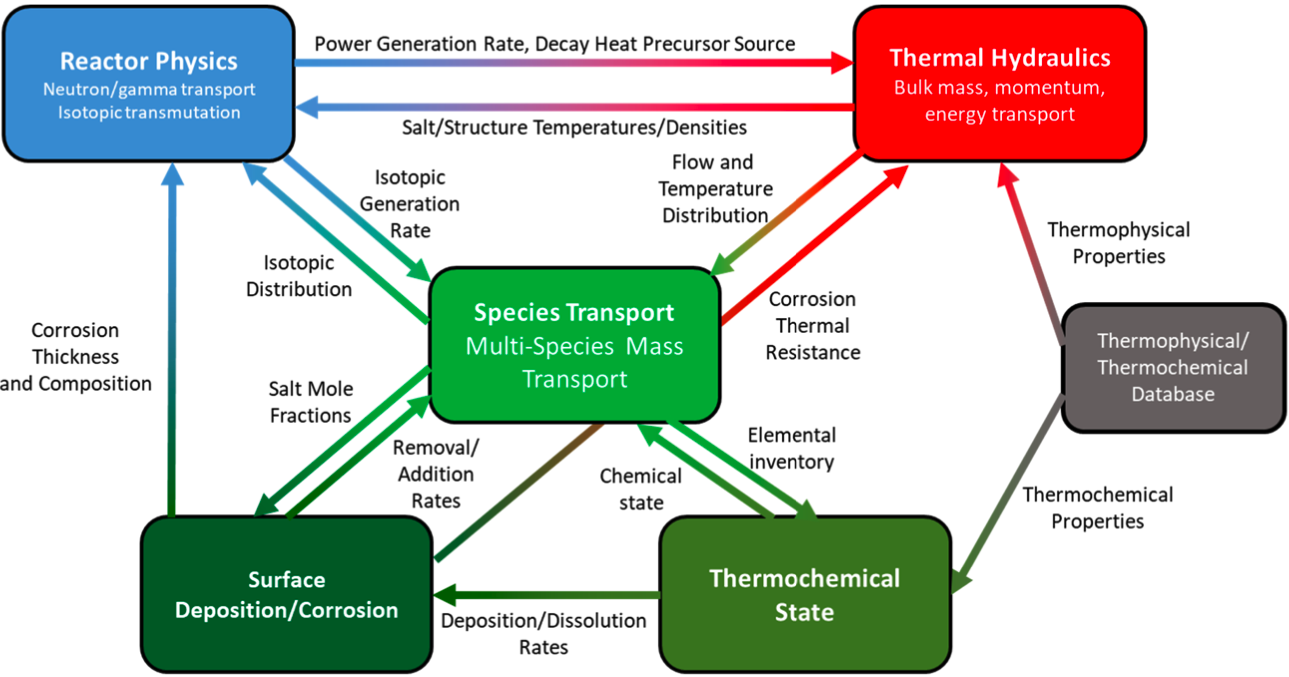
\includegraphics[width=0.75\textwidth]{figures/chapter-1/MSR_MP}
		\caption[Multiphysics phenomena in molten salt reactors (MSRs).]{Multiphysics phenomena in molten salt reactors (MSRs) \cite{McMurray:2021aa}.}
		\label{fig:msr_mf}
	\end{figure}
	
	 Evidently, modelling and simulation of nuclear materials requires a multiscale, multiphysics approach. However, such simulations have been decently challenging until recently and with significant limitations on the amount of computational resources available even a couple of decades ago, a majority of modelling and simulation efforts adopted an operator-splitting approach based on Picard iterations. Such simulations usually focussed on only the engineering scale behaviour and usually relied on continuum or bulk description of the phenomena. In doing so, experimental observations and operational experience were relied on for the validity of results and often very conservative safety margins were added to design parameters. As an example, nuclear fuel behaviour has been modelled as a solid mechanics problem coupled with conductive heat transfer and fission gas release wherein the material properties are often either assumed to be constant or described using simplified models based on empirical correlations. Though these methods were suitable for previous and current generation of nuclear reactors, addressing the materials challenges for advanced reactors is usually beyond their capability. In fact, there has been an increasing impetus on leveraging lower scale information to inform models on larger scales and solving the governing equations as a system rather than as individual problems.  Since such an approach is rooted in fundamental principles, the transfer of information between scales, through characteristic parameters such as density, energy, temperature, etc., results in a much more accurate description of material behaviour \cite{STAN200920}. The numerous modelling and simulation tools available at different length and time scales are shown in figure~\ref{fig:multiphys}.
	\begin{figure}[htb]
		\centering
		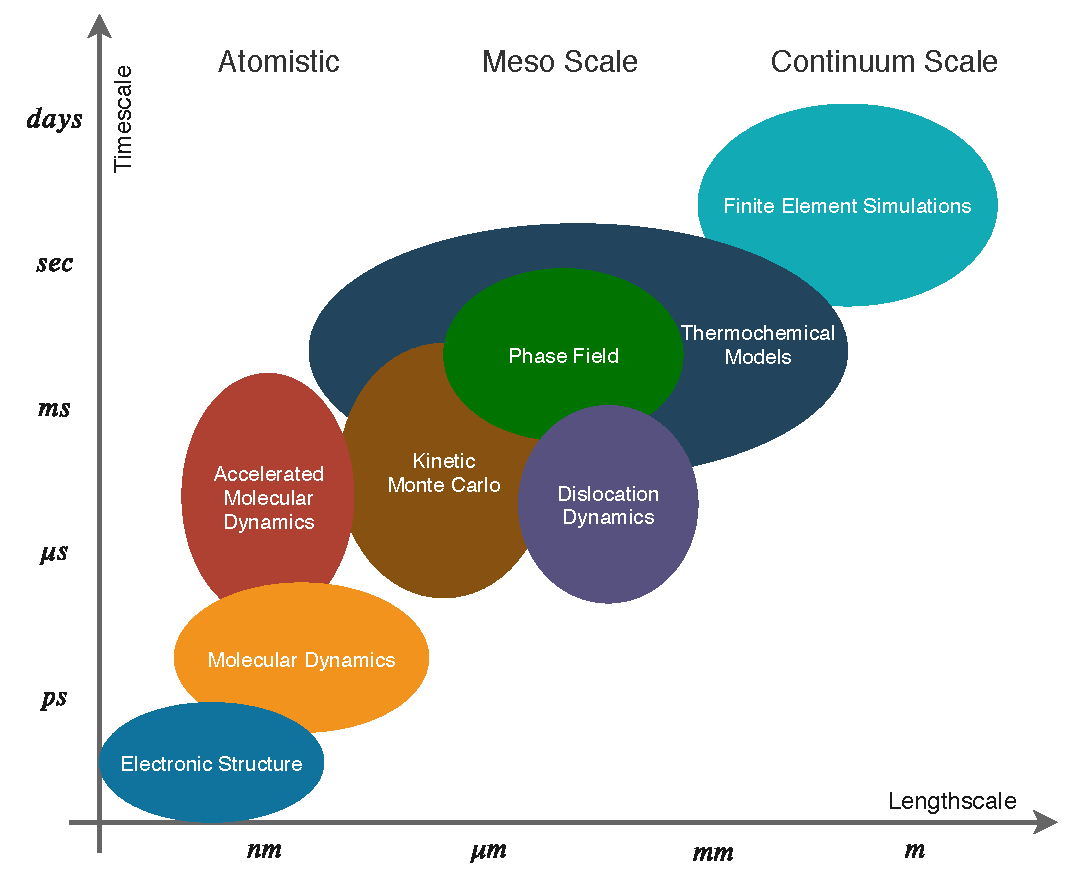
\includegraphics[width=0.75\textwidth]{figures/chapter-1/Multiphysics.pdf}
		\caption[Multiscale methods used for materials modelling simulation]{Multiscale theoretical and computational methods used for materials model development and computer simulation \cite{STAN200920}.}
		\label{fig:multiphys}
	\end{figure}
	
\subsection{Computational Thermodynamics}
	The modelling and simulation tool that is of particular relevance to this work is computational thermodynamics. Phase and chemical behaviour of nuclear materials is governed by the thermochemical equilibrium state and, though in many systems, equilibrium may not be achieved, a thorough understanding of both transport and chemical evolution, and subsequently material properties, is based on an accurate representation of thermochemical equilibria \cite{Devanathan:2010aa}. As an example, the oxygen chemical potential acts as the driving force for transport of oxygen in oxide fuels but a determination of these chemical potentials is impossible without determining the stable phases which depends on the oxygen-to-metal ratio which in turn is a function of burnup.  For such complex systems, computational thermodynamics is an essential tool for calculating both phase equilibria and thermodynamic properties of the system. Computational thermodynamics is rooted in the \emph{CALculation of PHAse Diagram} (CALPHAD) approach shown in figure~\ref{fig:calphad}. CALPHAD combines
 experimental and theoretical information and tunes parametric models to describe thermodynamic properties of materials like Gibbs energy, enthalpy, heat capacity, etc. \cite{Lukas07}.
	\begin{figure}[htb]
		\centering
		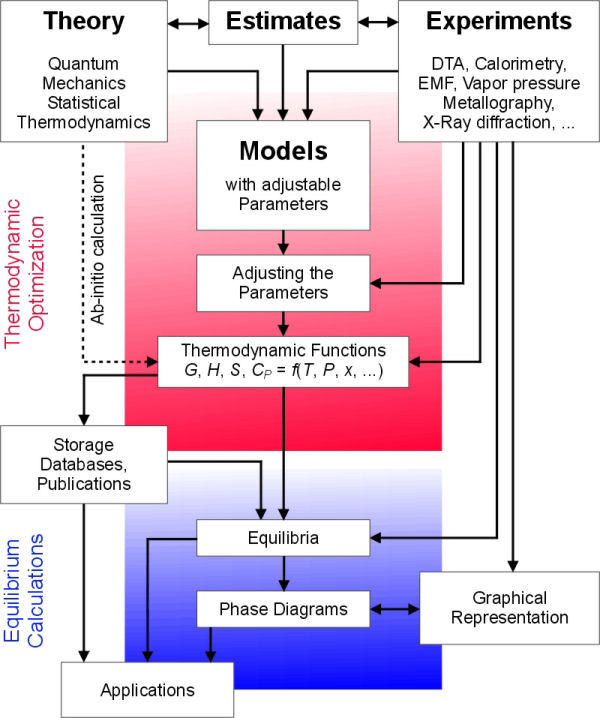
\includegraphics[width=0.6\textwidth]{figures/chapter-1/Calphad_method}
		\caption[Principle of CALPHAD method]{Principle of CALPHAD method by Zinkevich \cite{Zinkevich:2003aa}.}
		\label{fig:calphad}
	\end{figure}

	Capturing thermodynamic equilibria in multiphysics codes has traditionally relied on empirical correlations and the interest in direct coupling of thermodynamic equilibrium codes with multiphysics model is only a recent trend. While the empirical correlations do not convey the high fidelity of original thermodynamic analysis, performing thermodynamic equilibrium analysis within multiphysics codes is normally a very complex process and can significantly impede the computational performance of such codes. However, the recent developments in high performance computing have facilitated the use of equilibrium thermodynamics in multiphysics  simulations. Computational thermodynamics is of ever more importance in the discovery and design of materials for advanced reactors and is allowing phenomena hitherto not very well-understood even in current generation of reactors despite the years of experience.
	
	
	The inputs and outputs of thermodynamic equilibrium calculations are shown in figure~\ref{fig:Thermod}. Since thermodynamic equilibriums are isothermal and isobaric in nature, temperature and pressure are required as inputs along with the elemental composition of the material. While the equilibrium calculations are mathematically rigorous, they do require thermodynamic models of materials to describe some parameters. This makes computational thermodynamics partly-empirical in that the thermodynamic models are often created from experimental data but efforts to use atomistic calculations to inform and improvise the thermodynamic models are gaining traction. The results from equilibrium calculations include the stable phases, speciation of the stable phases, and several thermodynamic properties like Gibbs energy, chemical potentials, heat capacities, etc.
	\begin{figure}[ht]
        		\centering
        		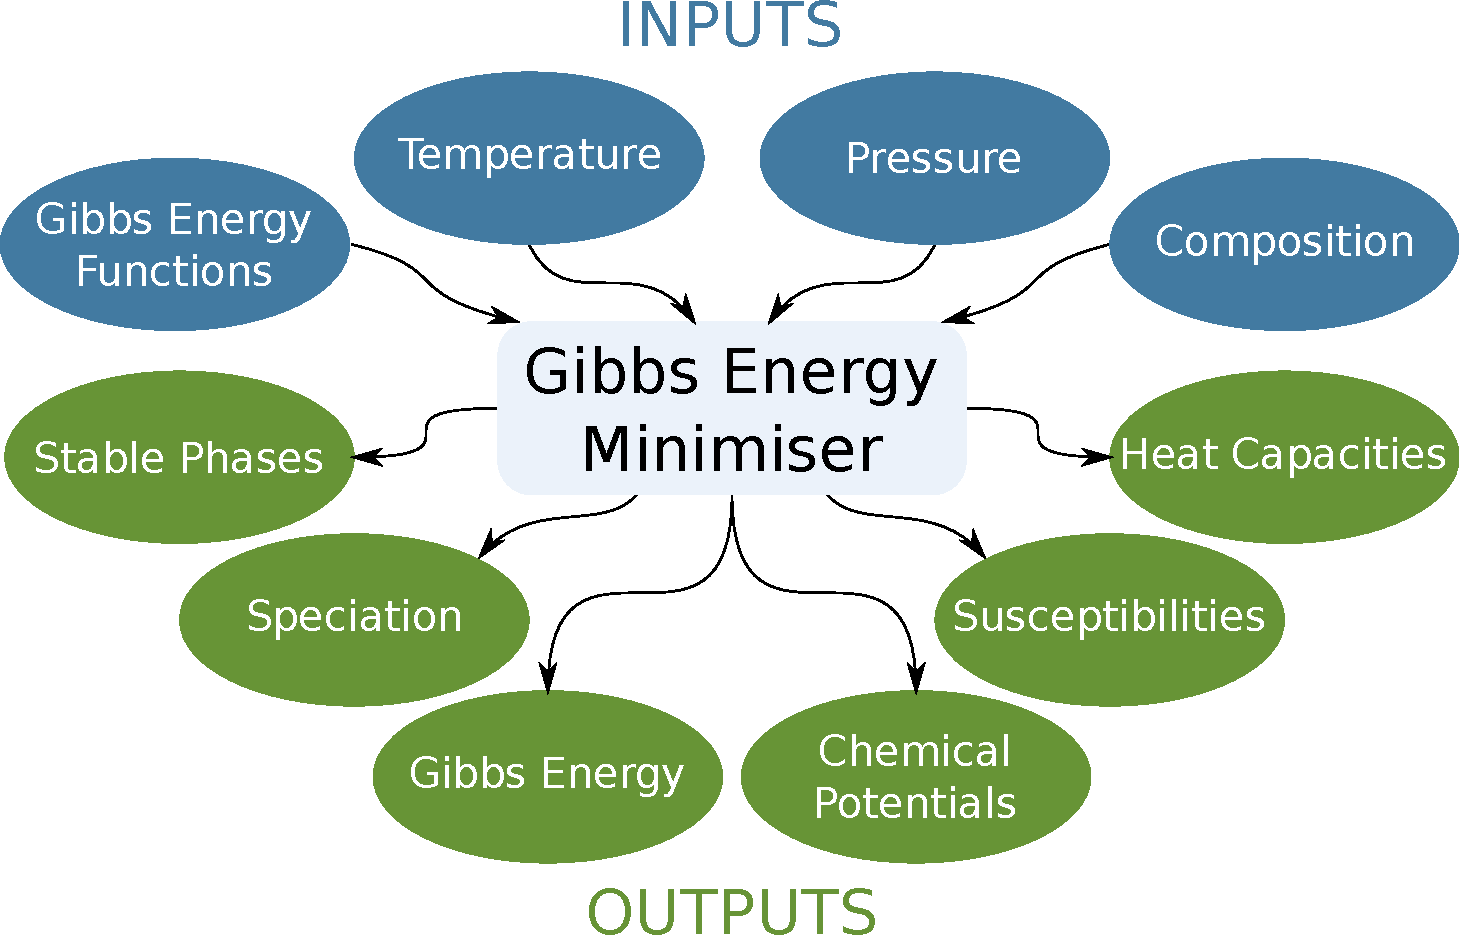
\includegraphics[width=0.75\textwidth]{figures/chapter-1/thermodynamics.pdf}
        		\caption{Input and output parameters of thermodynamic equilibrium calculations.}
        		\label{fig:Thermod}
    	\end{figure}
	
\subsection{Multiphysics Object Oriented Simulation Environment}
	The Multiphysics Object Oriented Simulation Environment (MOOSE) is a simulation framework that has been developed with the aim of harnessing modern massively parallel computing resources to perform complex multiphysics simulations. Exploiting the modern computational power is in itself a daunting task but the task of achieving complex simulations becomes ever more daunting for users when considerations such as numerical solve, discretisation of partial differential equations, etc. are added. The goal of MOOSE is to provide simplified interfaces for user facing tasks such as specification of partial differential equations, boundary conditions, material properties and all aspects of a simulation while handling complex background tasks such as parallel, adaptive, nonlinear, finite element solve internally \cite{Permann:2020aa}. Through the use of interfaces and inheritance, each portion of a simulation becomes reusable and an ecosystem for multiphysics simulations is formed allowing people from different groups and backgrounds to share code with growing capability. Originally created at the Idaho National Laboratory in the United States, MOOSE is open-source framework which leverages state-of-the-art libMesh code \cite{Kirk:2006aa} for finite elements and the Portable Extensible Toolkit for Scientific Computation (PETSc) \cite{Balay:2022ab,Balay:2022aa} for leading-edge numerical methods/solvers. MOOSE has been used to build multiple community-developed physics "modules" \cite{Guillaume:2021aa,Guillaume:2021ab,Adhikary:2016aa,Wilkins:2020aa,Shemon:2021aa} and several application libraries which are used by governments, industry and academia with applications ranging from nuclear fuel modelling to porous flow in 3D fractured porous media. MOOSE's capability is in contrast to what is often seen in commercial packages, where custom material models can limit the parallel scalability, forcing serial runs in the most severe cases \cite{gaston2015physics}. 
	
	For nuclear reactor modelling, apart from the MOOSE modules, several export-controlled applications have been developed. These include {RELAP-7} \cite{Zhang:aa} for system level thermal hydraulics, {Rattlesnake} \cite{Wang:aa} for neutronics, etc. For nuclear material simulations, the {MOOSE} framework consists of two main applications the macroscale fuel performance code {Bison} \cite{WILLIAMSON2012149} and the mesoscale phase field code {Marmot}  \cite{Tonks12}. 
	
	Simulation of nuclear reactor fuel performance involves complex thermomechanical processes between fuel pellets, made of fissile material, and the protective cladding barrier that surrounds the pellets. {Bison} is an engineering scale code developed to predict the nuclear fuel performance under normal, off-normal, and accident conditions. By using highly efficient computational methods, it enables three dimensional, fully coupled multiphysics simulations on high fidelity geometric representations of fuel pins/pellets. {Bison} has been designed to be highly scalable and does not require the use of operator splitting, staggered or predictor-corrector approaches \cite{WILLIAMSON2012149}.

	Due to its simple concept and large range of applicability, the phase field approach is a popular and powerful tool to model microstructure and has been applied in problems such as grain boundary migrations, martinistic transformation, two-phase flow, etc. The phase field approach treats all material interfaces as diffuse by representing structural features with continuous variables which smoothly transition from one value to another. Thus, phase field method not only eliminates the need to explicitly discretise boundaries and interfaces, it also enables describing microstructure through a system of partial differential equations.  The {Marmot} phase field application has been developed to enable simulations of the microstructure evolution of nuclear fuels and materials under irradiation. By exploiting the object-oriented architecture of {MOOSE}, {Marmot} allows easy coupling of phase field with additional physics such as solid mechanics or heat conduction, to effectively predict the microstructural evolution at mesoscale. This allows prediction of evolution of material properties of nuclear materials under irradiation and can be used to inform engineering scale simulations and reduce the dependence of such simulations on empirical correlations. As a result, the multiscale framework can achieve true predictability even in compositional and operational regimes where little or no experimental data exists.

	The software developed as part of this work adds native  equilibrium thermodynamic capability to MOOSE and its applications.

%==============================================================================================================================
%															Molten Salt Corrosion
%==============================================================================================================================	
\subsection{Yellowjacket}
	Many emerging nuclear technologies, such as MSRs, use high temperature fluids like molten fluoride/chloride salts, which can lead to the corrosion of salt-facing structural materials. Not only does corrosion impact the performance of structural materials with the possibility of compromising their integrity but it can also lead to other problems just as blocking of salt flow loops due to leaching from hot sections of the loop and deposition in the colder sections. Molten salt corrosion is fundamentally different from corrosion in LWRs, where oxidation leads to formation of a passive oxide layer creating a self-healing mechanism, and most of the methods to control corrosion developed over previous centuries are of limited value \cite{Yoshioka:2017aa}. In molten fluoride salts, the protective oxide layer on alloys typically relied upon for high-temperature corrosion resistance dissolves, thereby exposing the fresh alloy surface to the molten salt. In molten chloride salts, passivity has been observed; however, the oxide layer is prone to attack and may not provide the necessary corrosion protection \cite{Sridharan:2013aa}. The corrosion process is accelerated by the impurities present in the salt and enhanced further by the presence of dissimilar metals due to activity-driven corrosion. It has been observed the corrosion in molten salt is a microstructural phenomena with preferential leaching at grain boundaries as compared to bulk of the grain but there are significant gaps in the scientific understanding of the governing mechanisms such as the impact of impurities and irradiation \cite{Zheng:2018aa,Zhou:2020aa,Zhu:2021aa,Raiman:2018aa,Pillai:2021aa,Guo:2018aa}.
	
	Corrosion is an electrochemical process composed of oxidation and reduction reactions, which are defined by the thermodynamics and kinetics of the system. While thermodynamics controls whether or not a material may corrode, kinetics influences how quickly the material will corrode. This corrosion behaviour is also significantly affected by the material microstructure and predicting corrosion therefore requires a multiphysics approach that can couple quantitative electrochemistry models of corrosion and chemical reactions with thermochemical equilibrium computations. Effectively, predicting corrosion and related phenomena like leaching and deposition requires a multiscale, multiphysics approach \cite{Mcmurray:2018aa}. However, there has been a lack of dedicated tools for modelling molten salt corrosion and to bridge this gap, a suite of tools have been developed under the Nuclear Energy Advanced Modelling and Simulation (NEAMS) program of the United States Department of Energy (US-DOE). The goal of this suite, shown in figure~\ref{fig:yj_suite}, is to couple atomistic and mesoscale modelling to thermochemical equilibrium calculations to create a unique corrosion modelling capability on the microstructural scale and use it to inform engineering scale codes aimed at solving species transport problem. At the core of the corrosion suite is the MOOSE-based application {\YJ} that couples quantitative models of corrosion with thermodynamic equilibrium and chemical kinetics models to predict the rate of material loss, corrosion product production and precipitate production in advanced nuclear reactors. {\YJ} relies on the phase field method for structural evolution and couples it with electrochemical descriptions, fracture models and thermochemical equilibrium solver to create a holistic environment for corrosion modelling and simulation \cite{Bhave:2022aa}.
	\begin{figure}[htb]
		\centering
		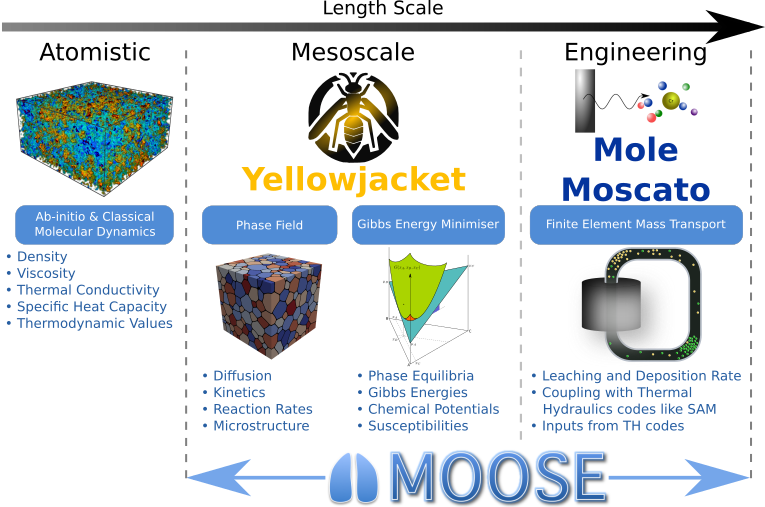
\includegraphics[width=0.9\textwidth]{figures/chapter-1/Yellowjacket_Suite.png}
		\caption{{\YJ} corrosion suite.}
		\label{fig:yj_suite}
	\end{figure}

	In the case of {\YJ}, as shown in figure~\ref{fig:yj_io}, the phase field model requires several thermodynamic properties like Gibbs energies, chemical potentials and driving forces for the various phases which can be present in the system. This requires knowing the molar amounts of the different phases which would be present under given temperature, pressure and composition. However, at the interfaces, more than one phase can co-exist and the phase field models face a challenge in estimating the assemblage and thermodynamic properties. In such cases, a thermodynamic equilibrium solver can provide the required information to the phase field module. This is the prime driving force behind the development of {\GEM}. One may argue that the system will not be at equilibrium and that kinetics of the system will drive the corrosion behaviour and therefore might question the appropriateness of thermochemical equilibrium calculations. While the system is not really at equilibrium, it can be safely assumed that in the limiting case the system will be at equilibrium at any point in space and time.
	\begin{figure}[htb]
		\centering
		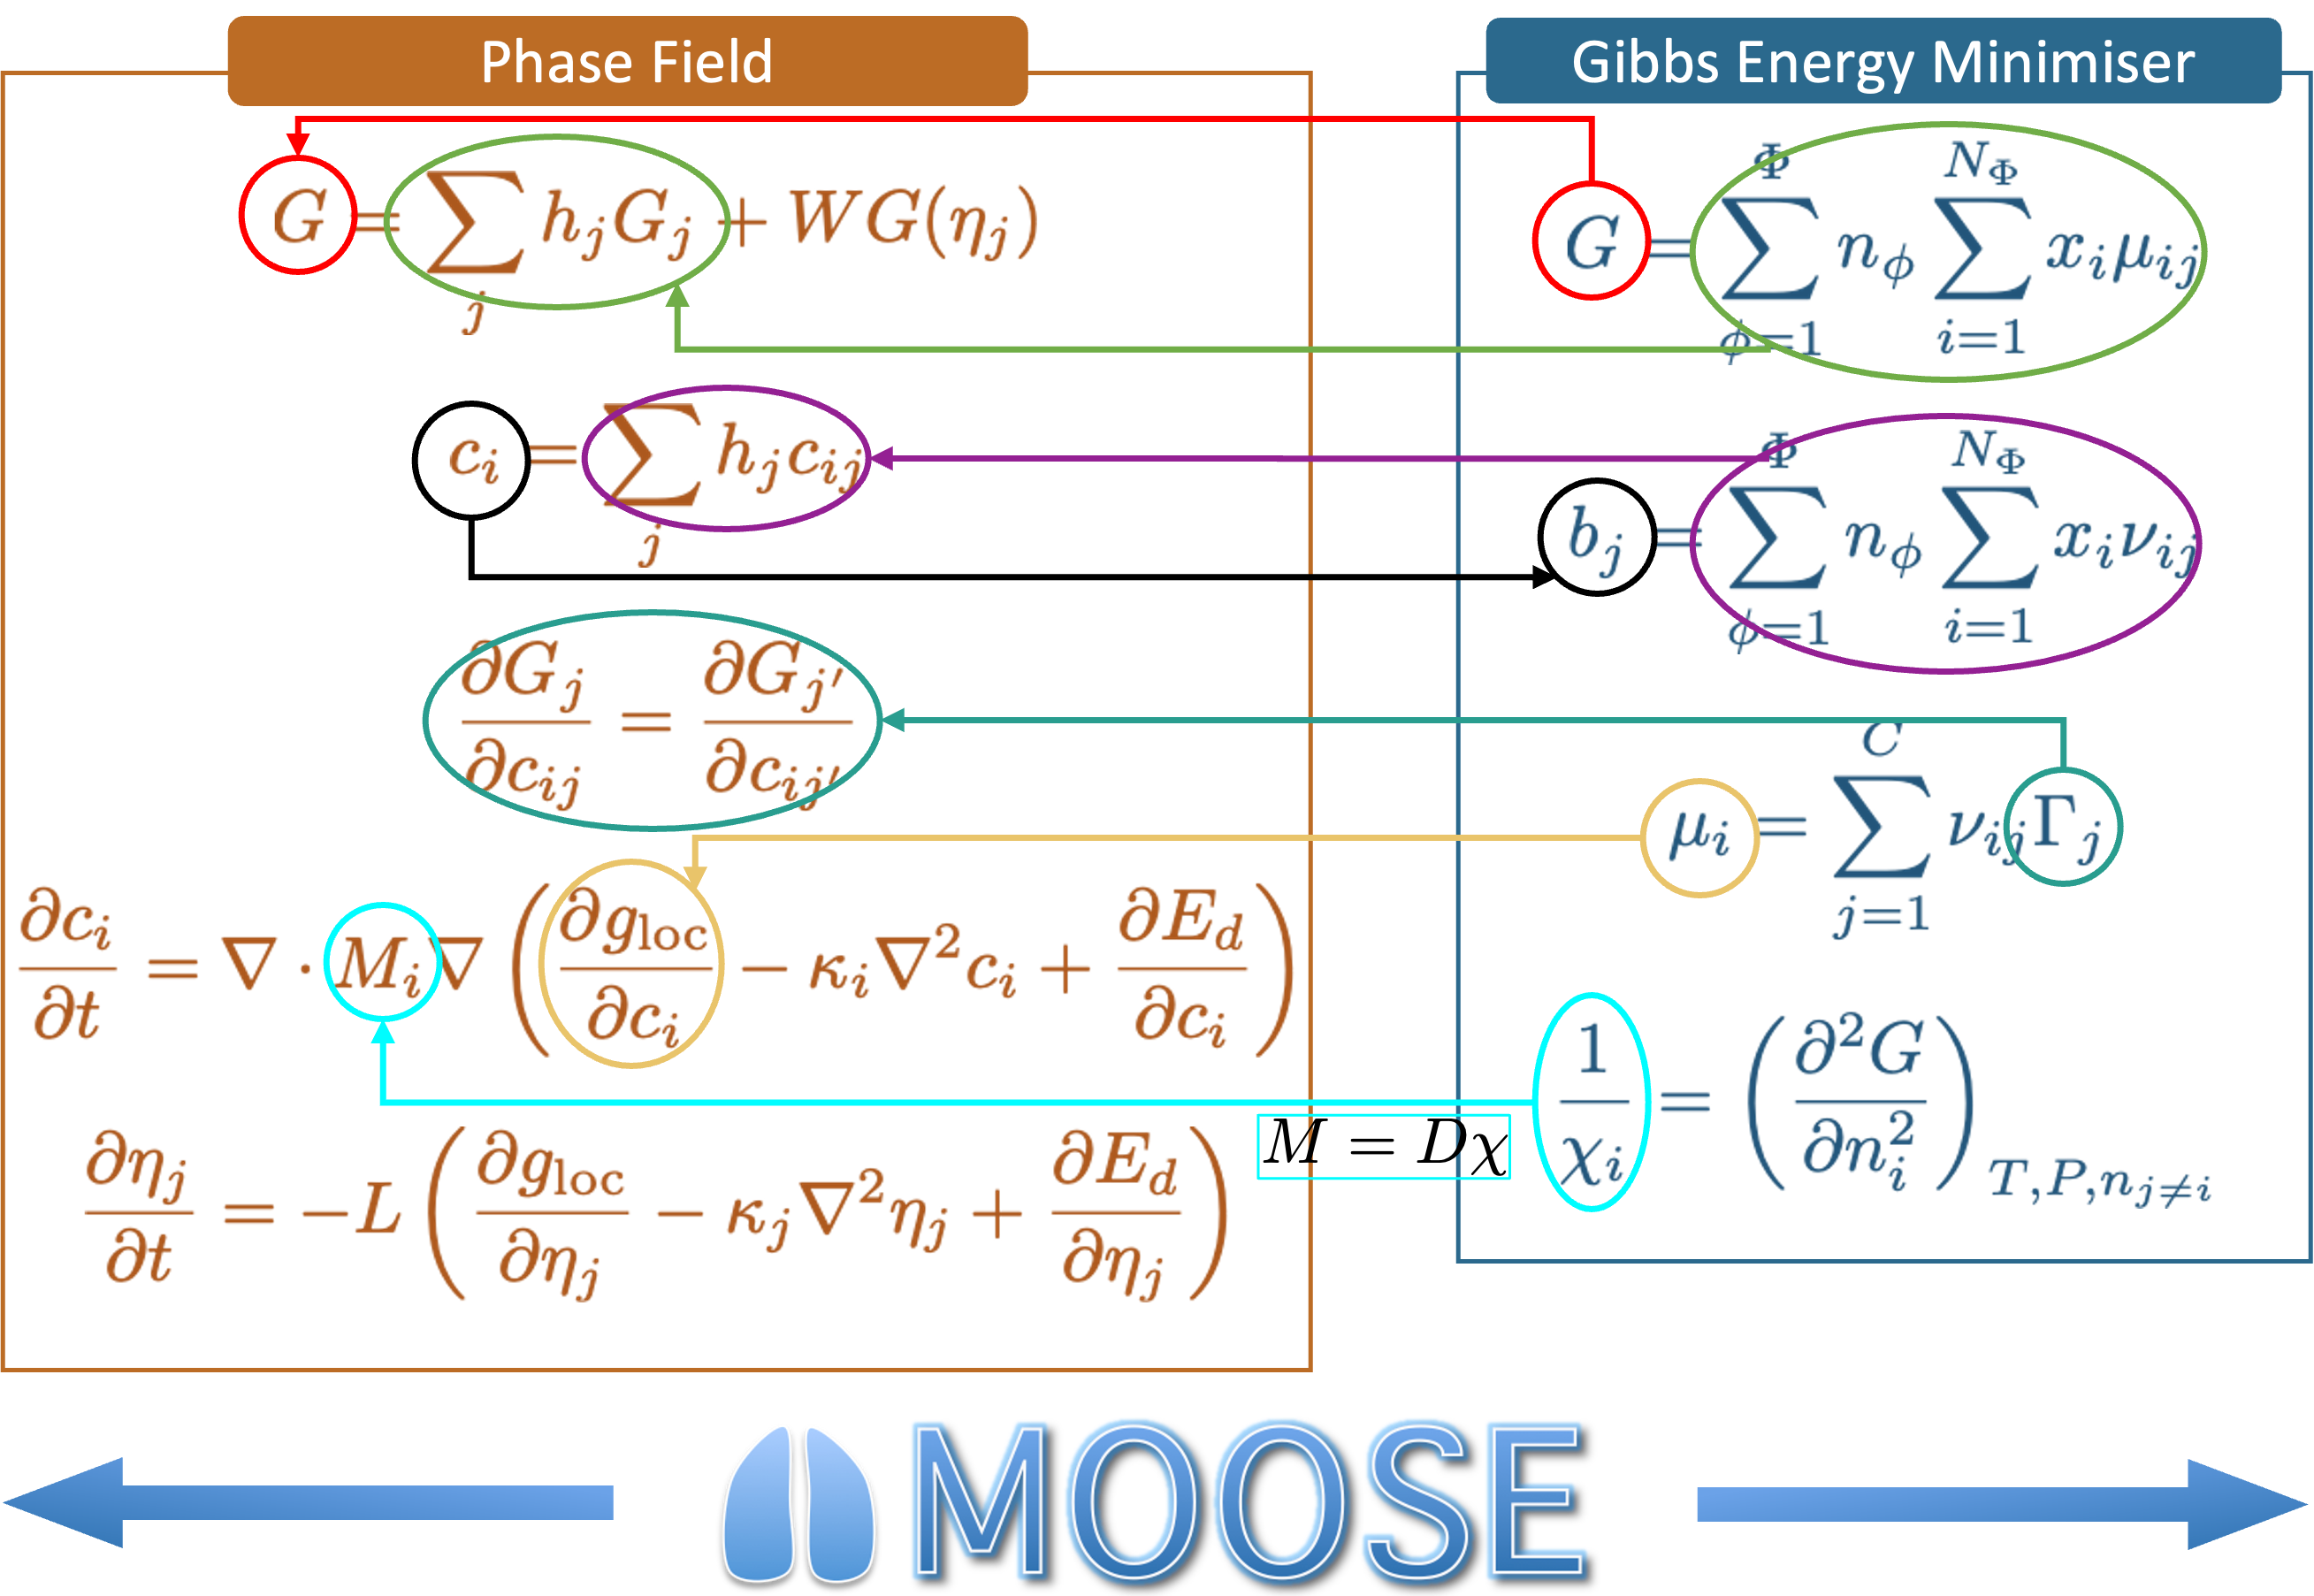
\includegraphics[width=0.8\textwidth]{figures/chapter-1/YJ_PF_IO.png}
		\caption{Information exchange between the phase field and equilibrium thermodynamics modules of \YJ.}
		\label{fig:yj_io}
	\end{figure} 	

	{\YJ} is multi-institutional collaborative effort between the Idaho National Laboratory, University of Florida, and Ontario Tech University.  In {\YJ}, the phase field module was implemented at University of Florida, computational thermodynamics development was performed as part of this PhD thesis at Ontario Tech University and MOOSE-integration was primarily done at Idaho National Laboratory. The main motivation behind this work was to enable direct coupling of thermodynamic equilibrium calculations in MOOSE-based multiphysics simulation and a new Gibbs energy minimiser called {\GEM} and the objectives, tasks and main outcomes are described in the next chapter.
	
	
	The rest of this thesis is organised as follows: the motivation, objectives and deliverables are summarized in \nameref{chap:overview}. A comprehensive literature review of the current computational thermodynamics methods and codes, and global optimisation tools for phase equilibria is provided in \nameref{chap:litreview}.  Then, the basic thermodynamics principles that form the basis of this work are described in \nameref{chap:thermo}. Conditions of phase equilibrium and the methods for computing them are described in \nameref{chap:equilibrium} and their implementation in {\GEM} is discussed in \nameref{chap:implementation}. To highlight the capability and potential impact of the developed tool, several applications of {\GEM} are shown in \nameref{chap:results}, which is followed by the \nameref{chap:conclusions} and \nameref{chap:future}. 